\chapter{GUI dell'app}

\section{Avvio dell'app}
\begin{figure}[ph]
	\centering
	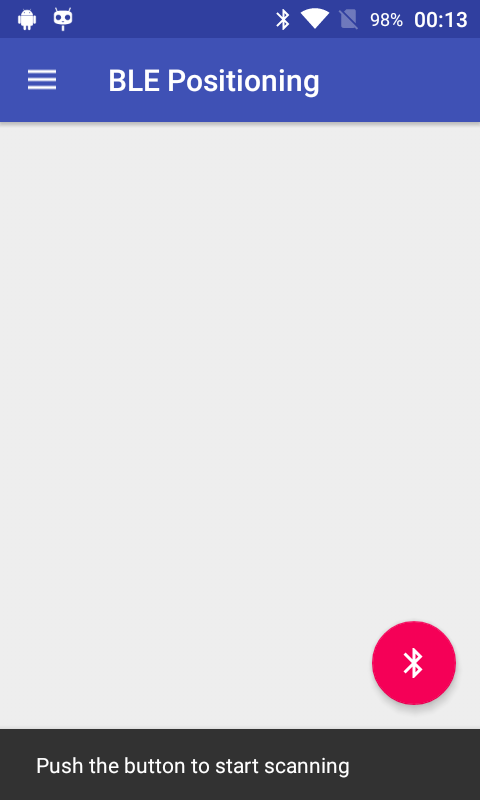
\includegraphics[width=.35\linewidth]{img/app/01.png}
	\caption{}
\end{figure}

\newpage
\section{Abilitazione dellla radio Bluetooth}
\begin{figure}[ph]
	\centering
	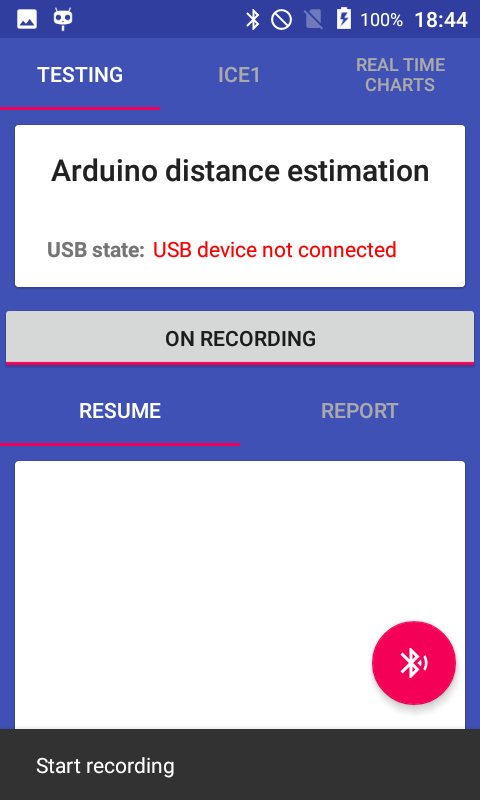
\includegraphics[width=.35\linewidth]{img/app/12.png}
	\caption{}
\end{figure}

\newpage
\section{Scansione dei dispositivi}
\begin{figure}[ph]
	\centering
	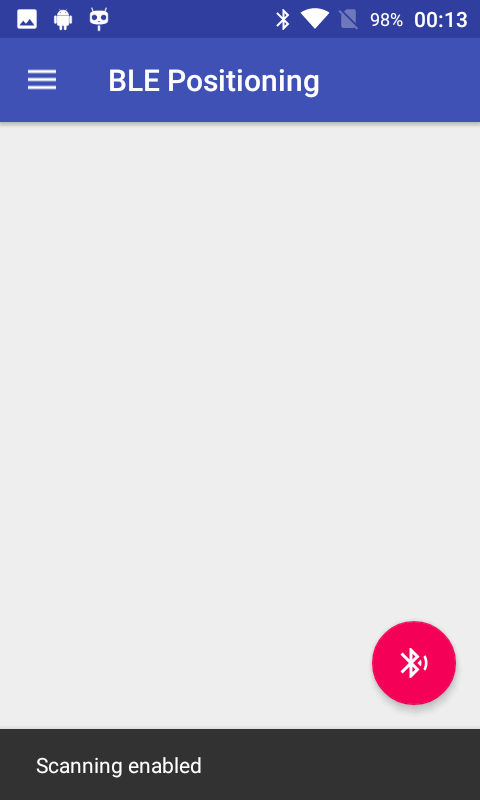
\includegraphics[width=.35\linewidth]{img/app/02.png}
	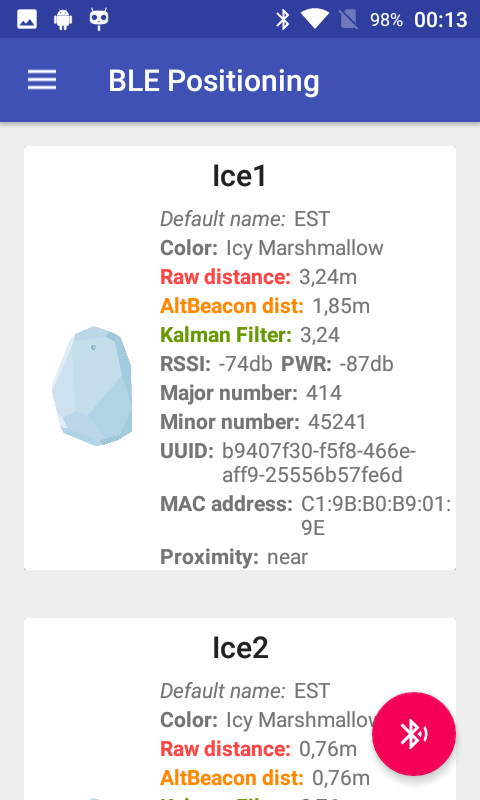
\includegraphics[width=.35\linewidth]{img/app/03.png}
	\caption{}
\end{figure}

\newpage
\section{Menù a sinistra}
\begin{figure}[ph]
	\centering
	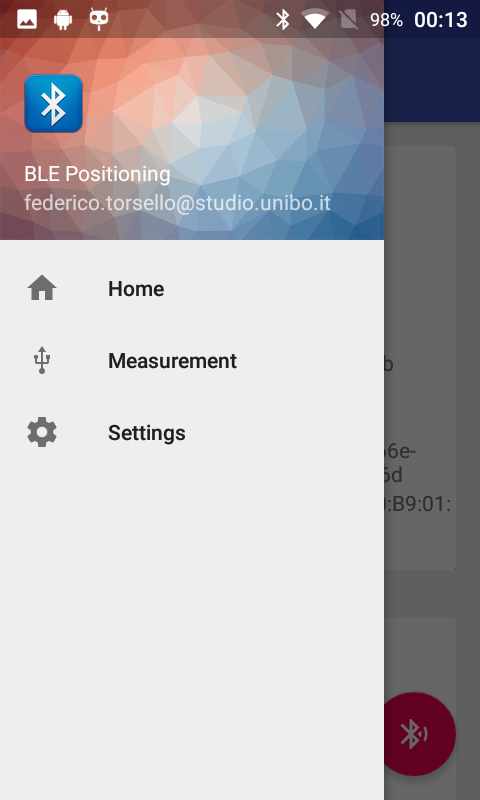
\includegraphics[width=.35\linewidth]{img/app/04.png}
	\caption{}
\end{figure}

\newpage
\section{Menù a destra}
\begin{figure}[ph]
	\centering
	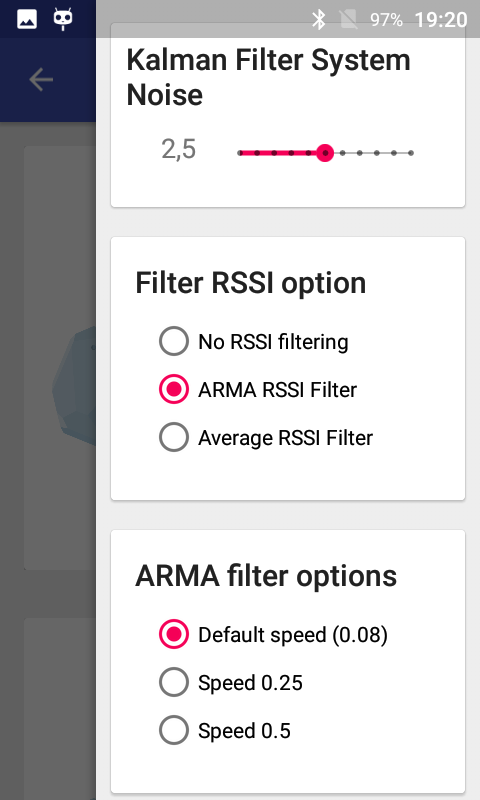
\includegraphics[width=.35\linewidth]{img/app/05.png}
	\caption{}
\end{figure}

\newpage
\section{Dettagli di un dispositivo}
\begin{figure}[ph]
	\centering
	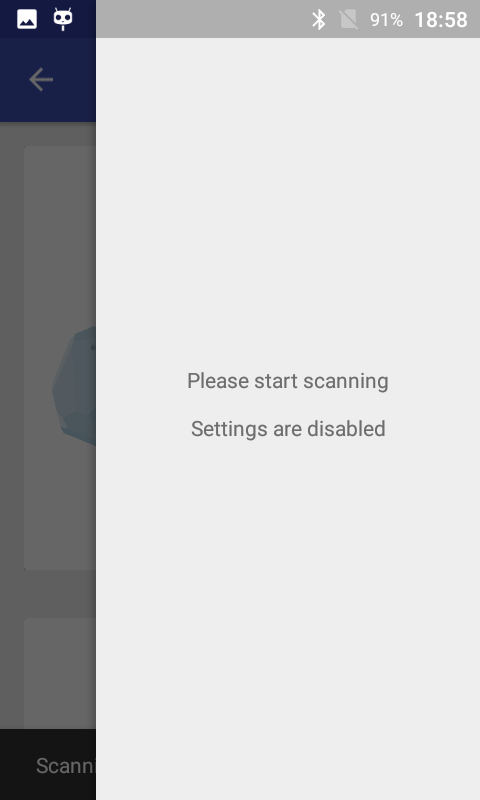
\includegraphics[width=.35\linewidth]{img/app/06.png}
	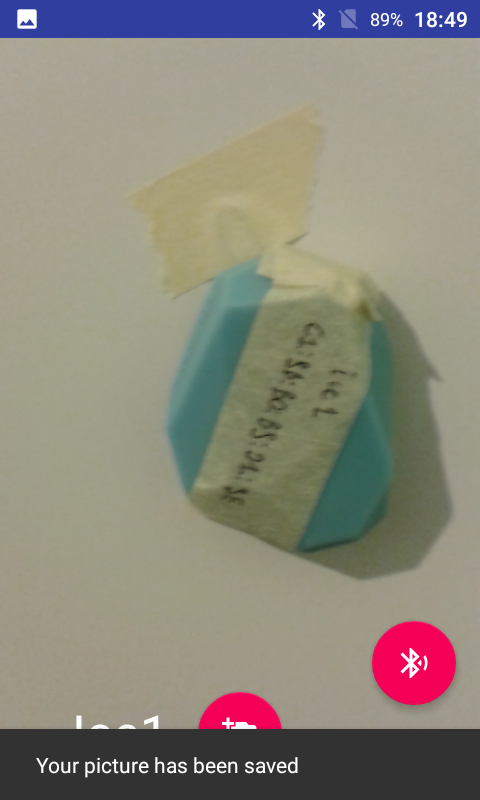
\includegraphics[width=.35\linewidth]{img/app/07.png}
	\caption{}
\end{figure}

\newpage
\section{Dettagli avanzati e grafici realtime}
\begin{figure}[ph]
	\centering
	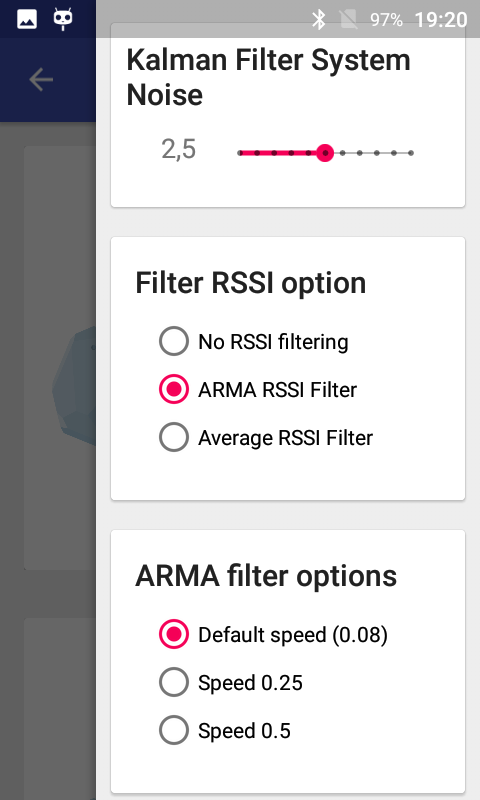
\includegraphics[width=.35\linewidth]{img/app/08.png}
	\caption{}
\end{figure}

\newpage
\section{Connessione con Arduino via USB OTG}
\begin{figure}[ph]
	\centering
	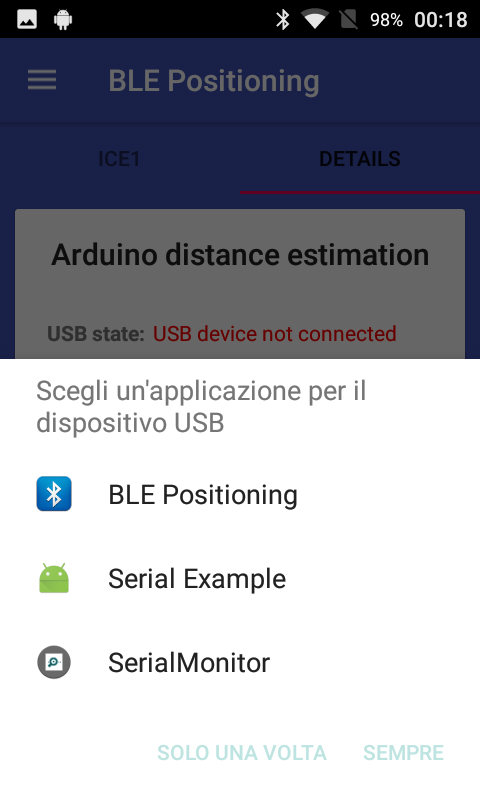
\includegraphics[width=.35\linewidth]{img/app/09.png}
	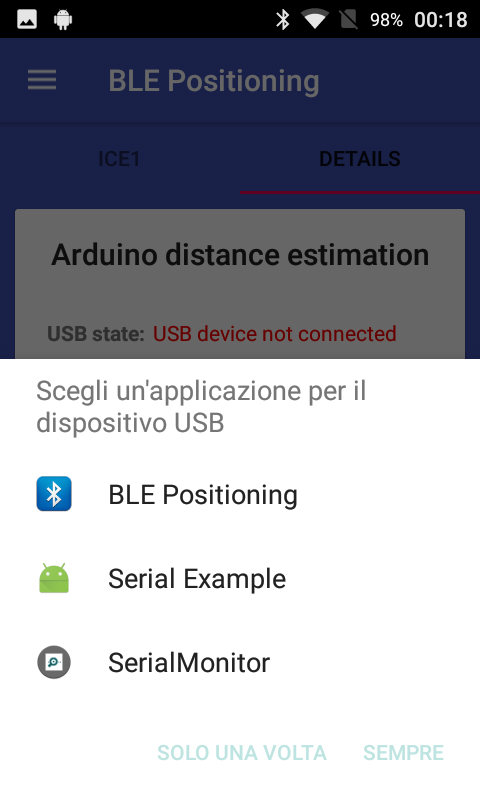
\includegraphics[width=.35\linewidth]{img/app/10.png}
	\caption{}
\end{figure}

\newpage
\section{Feedback della stima della distanza con Arduino}
\begin{figure}[ph]
	\centering
	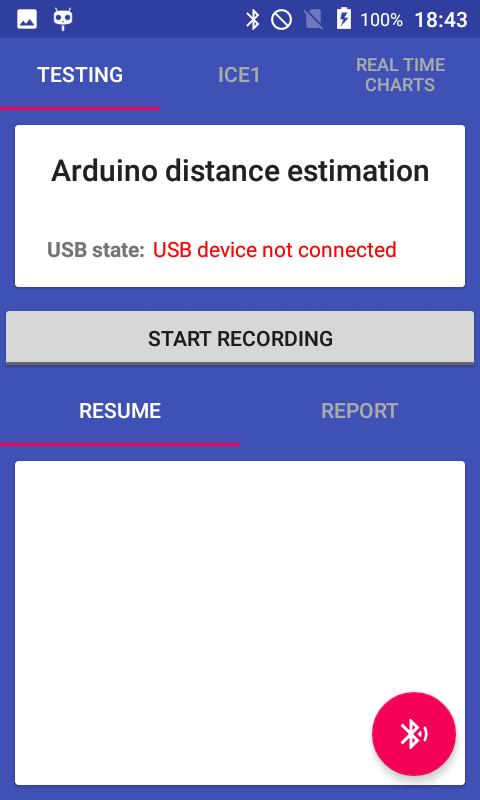
\includegraphics[width=.35\linewidth]{img/app/11.png}
	\caption{}
\end{figure}